\documentclass{beamer}
\usepackage{amsmath}
%\usepackage{beamerthemesplit} % new 
\usetheme{Madrid}
\usefonttheme[onlymath]{serif}
\setbeamertemplate{frametitle}[default][center] %center slide titles

\begin{document}
\title{Notes on Siemens Ch. 3}
\author{Cody Petrie} 
\date{\today} 

%start slides
\frame{\titlepage} 

\frame{\frametitle{The Black Sphere}
\begin{itemize}
   \item Model neutron scattering from nuclei as a particle being absorbed by spherical object.
   \item Start by expanding an incident plane wave in terms of spherical harmonics.
   \begin{align}
      e^{i\mathbf{k}\cdot\mathbf{r}} &= \sum\limits_l C_l Y_l^0(\theta) \\
      e^{ikz} &\approx \sum\limits_l \frac{\sqrt{\pi}}{kr} \sqrt{2l+1} \, i^{l+1} \left( e^{-i(kr-\frac{l\pi}{2})} - e^{i(kr-\frac{l\pi}{2})} \right) Y_l^0(\theta)
   \end{align}
   \item Here we have used the fact that $\mathbf{k}\cdot\mathbf{r}$ only depends on $\theta$, and not on $\phi$, thus $m=0$. Also, we have used various identities and the orthonormality of spherical harmonics.
\end{itemize}
}

\frame{\frametitle{The Black Sphere}
\begin{itemize}
   \item Scattering only happens for short time
   \begin{equation}
      \phi(r\rightarrow\infty) = \sum\limits_l \frac{\sqrt{\pi}}{kr} \sqrt{2l+1} \, i^{l+1} \left( e^{-i(kr-\frac{l\pi}{2})} - \eta_l e^{i(kr-\frac{l\pi}{2})} \right) Y_l^0(\theta)
   \end{equation}
   \item Scattered wave is just the total wave function minus the incident wave function, $\phi_{sct} = \phi(r\rightarrow\infty) - e^{ikz}$.
   \begin{equation}
      \phi(r\rightarrow\infty) = e^{ikz} + f(\theta)\frac{e^{ikr}}{r}
   \end{equation}
   \begin{equation}
      f(\theta) = \sum\limits_l i \frac{\sqrt{\pi}}{k}\sqrt{2l+1} Y_l^0(\theta) (1-\eta_l)
   \end{equation}
   \item This looks like a scattering amplitude, $\frac{d\sigma}{d\Omega} = |f(\theta)|^2$.
\end{itemize}
}

\frame{\frametitle{The Black Sphere}
\begin{itemize}
   \item \textbf{Approximations:} Classical turning point is where $k^2 = l(l+1)/R^2 \approx (l+\frac{1}{2})^2/R^2$. If particle passes inside the range of force ($R$) you get absorption ($\eta_l = 0$), but if not you get none ($\eta_l = 1$).
   \begin{equation}
      \frac{d\sigma}{d\Omega} = \frac{\pi}{k^2} \left|\sum\limits_{l=0}^{kr-1/2} \sqrt{2l+1} Y_l^0(\theta)\right|^2
   \end{equation}
   \item \textbf{More Approximations:} Here we approximate this for large and small angle scattering. I was not able to figure out the integrals so I'll just quote their answer here.
   \begin{align}
      \frac{d\sigma}{d\Omega} \approx
   \begin{cases}
      \frac{2R}{\pi} k\theta^2 \sin\theta\cos^2\left(kR\theta+\frac{\pi}{4}\right),& \text{for } kR\theta \gg 1 \\
      \frac{k^2R^4}{4}(1-(kR\theta/2)^2)^2,& \text{for } kR\theta \ll 1
   \end{cases}
   \end{align}
\end{itemize}
}

\frame{\frametitle{The Black Sphere}
\begin{figure}[h]
   \centering
   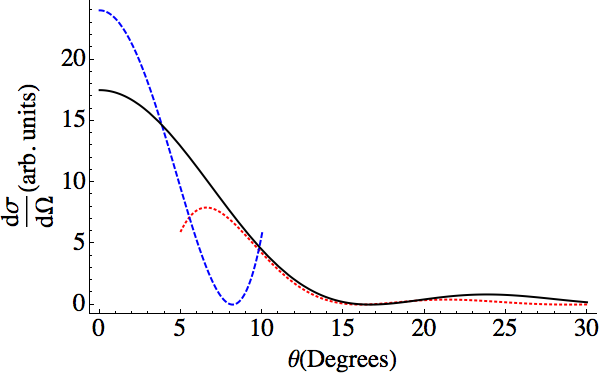
\includegraphics[width=0.4\textwidth]{../fig3_2.png}
   \caption{Rough reproduction of figure 3.2 in the book.}
\end{figure}
\begin{itemize}
   \item To find the angle of minumum scattering I have taken the derivative of the high angle scattering and set it equal to zero to get.
   \begin{equation}
      \theta_{min} = \frac{\pi}{4kR}(2n-1)
   \end{equation}
   \item Experiment must show that it's actually
   \begin{equation}
      \theta_{min} = \frac{5\pi}{4kR}
   \end{equation}
\end{itemize}
}

\frame{\frametitle{The Black Sphere}
\begin{equation}
   \theta_{min} = \frac{5\pi}{4kR}
\end{equation}
\begin{itemize}
   \item Now we can use this diffraction pattern to estimate the radius of nuclei. For Pb with $\epsilon = 84$ MeV we get $k = \sqrt{2m_N\epsilon/\hbar} \approx 2.0$ fm$^{-1}$. Now the graph above shows that $\theta_{min} \approx 15^\circ$. This gives us a radius of 7.5 fm.
   \item A quick google search gives Pb a radius of 7 fm.
\end{itemize}
}

\frame{\frametitle{Nuclear Sizes and Saturation}
\begin{columns}[onlytextwidth]
\begin{column}{0.25\textwidth}
   \centering
   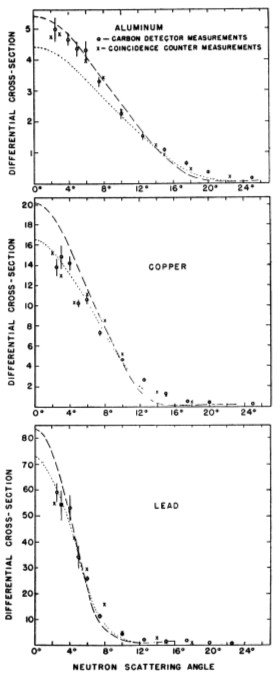
\includegraphics[scale=0.46]{../fig3_1.jpg}
\end{column}
\begin{column}{0.75\textwidth}
   \begin{itemize}
      \item You can see from this that the volume $\Omega_r \propto \theta_{min}^{-3}$, so the smaller the nuclei the bigger the scattering angles.
      \item Coupled with figure 3.1 in the book which shows that lighter nuclei have larger scattering angles this shows that lighter nuclei are smaller than heavier nuclei.
      \item In fact it turns out that
      \begin{equation}
         \Omega_r = \Omega_0 A
      \end{equation}
      \begin{equation}
         R = r_0 a^{1/3}
      \end{equation}
      with $r_0 \approx 1.3$ fm and $\Omega_0 = \frac{4}{3}\pi r_0^3 \approx 9$ fm$^3$.
   \end{itemize}
\end{column}
\end{columns}
}

\frame{\frametitle{Optical Model}
\begin{itemize}
   \item Compare this black sphere model to the potential model with a nice Hermitial potential
   \begin{equation}
      H = \frac{\mathbf{p}^2}{2m_N}+U(\mathbf{r}).
   \end{equation}
   \item Let's compare this to the black sphere model. Experiment tells us that $\sigma_{el}$ and $\sigma_{abs}$ should be comparable, where.
   \begin{equation}
      \sigma_{tot} = \sigma_{el} + \sigma_{abs}
   \end{equation}
   \begin{align}
      \sigma_{el} = \int d\Omega \left(\frac{d\sigma}{d\Omega}\right)_{el} &= \frac{\pi}{k^2}\sum\limits_{l=0}^\infty(2l+1)\left|1-\eta_l\right|^2 \\
      \sigma_{abs} &= \frac{\pi}{k^2}\sum\limits_{l=0}^\infty(2l+1)\left(1-|\eta_l|^2\right)
   \end{align}
\end{itemize}
}
\frame{\frametitle{Optical Model}
\begin{align}
   \sigma_{el} = \int d\Omega \left(\frac{d\sigma}{d\Omega}\right)_{el} &= \frac{\pi}{k^2}\sum\limits_{l=0}^\infty(2l+1)\left|1-\eta_l\right|^2 \\
   \sigma_{abs} &= \frac{\pi}{k^2}\sum\limits_{l=0}^\infty(2l+1)\left(1-|\eta_l|^2\right)
\end{align}
\begin{itemize}
   \item For the black sphere model ($\eta_l = 0, 1$)
   \begin{equation}
      \sigma_{el} = \sigma_{abs} = \pi R^2 ~ \mathrm{or} ~ 0
   \end{equation}
   \item For the potential model
   \begin{align}
      \sigma_{abs} = 0
   \end{align}
\end{itemize}
}

\frame{\frametitle{Optical Model}
\begin{itemize}
   \item However we can alter the potential model (not Hermitian anymore, losing C.M. energy particles)
   \begin{equation}
      H = \frac{\mathbf{p}^2}{2m_N}+U(\mathbf{r}) - iW(\mathbf{r})
   \end{equation}
   \item Solving the Schr\"odinger eq. for a stream of particles of energy $\epsilon$ moving in the $x$ direction we get
   \begin{equation}
      \phi(\mathbf{r},t) = \mathrm{const} \times e^{(ik-\kappa)x} e^{-i\epsilon t/\hbar}
   \end{equation}
   \begin{equation}
      \frac{\hbar^2}{2m_N}(k^2-\kappa^2) = \epsilon - U
   \end{equation}
   \begin{equation}
      \frac{\hbar^2}{m_N}\kappa k = W
      \label{eq:Wwithkappa}
   \end{equation}
\end{itemize}
}

\frame{\frametitle{Optical Model}
\begin{itemize}
   \item Now you can look at probability density and see how fast it attenuates.
   \begin{equation}
      \left|\phi(\mathbf{r})\right|^2 \sim e^{-2\kappa x}
   \end{equation}
   \item This gives us a mean free path for absorption of a nucleon of (falls of by factor $1/e$)
   \begin{equation}
      \lambda = \frac{1}{2\kappa}.
      \label{eq:meanfreepath}
   \end{equation}
   \item This will be used later.
\end{itemize}
}

\frame{\frametitle{Optical Model}
\begin{itemize}
   \item Now if we add in the main spin dependant effect we get the \textbf{Phenomenologibal Optical Model}.
   \begin{equation}
      H^{POM}=\frac{\mathbf{p}^2}{2m_H} + U(r) + \mathbf{l}\cdot\mathbf{s}U^{ls}(r) - iW(r)
   \end{equation}
   \item Fitting the results to various forms for thse potentials shows that the following gives good results.
   \begin{align}
      U(r) &= U_0f((r-R(A))/a_u)+U_C(r) \\
      W(r) &= \left(W_0-4W_1a_W\frac{\partial}{\partial r}\right)f((r-R(A))/a_W) \\
      U^{ls}(r) &= U^{ls}_0\frac{1}{r}\frac{\partial}{\partial r}f((r-R(A))/a_{ls})
   \end{align}
\end{itemize}
}

\frame{\frametitle{Optical Model}
\begin{itemize}
   \item See the book for constants. The $f$ is called the Woods-Saxon shape.
   \begin{equation}
      f(x) = (1-\exp(x))^{-1},~ x = (r-R(A))/a_U 
   \end{equation}
   \begin{figure}[h]
      \centering
      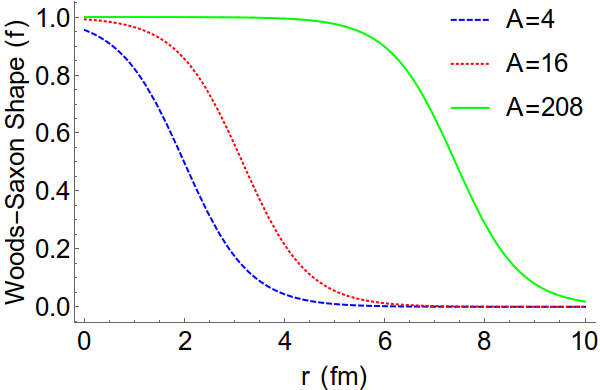
\includegraphics[width=0.4\textwidth]{../woodssaxon.png}
%      \caption{Woods-Saxon shape for various A.}
   \end{figure}
   \item The key features are that it approaches 1 inside the nucleus and falls from 0.9 to 0.1 as $r$ varies from $R - 2.2a_U$ to $R + 2.2a_U$. Surface thickness of $4.4a_U$ or 2.9 fm, about the range of the force.
\end{itemize}
}

\frame{\frametitle{Optical Model}
\begin{itemize}
   \item It is interesting to note that some of these potentials depend on the energy of the incident nucleon ($\epsilon$). The more energetic the more likely to be absorbed by exciting another nucleon.
   \begin{align}
      W_0(\epsilon) &\approx \max (0.22\epsilon - 2\mathrm{MeV},0) \\
      W_1(\epsilon) &\approx \max \left[12\mathrm{MeV} - 0.25\epsilon + 24\mathrm{MeV} \cdot t_3\frac{N-Z}{A},0\right] \\
      U_0(\epsilon) &\approx -50\mathrm{MeV}-48\mathrm{MeV}\cdot t_3\frac{N-Z}{A}+0.3(\epsilon-U_C(R)) \\
      U_0^{ls} &\approx 30\mathrm{MeV fm^2/\hbar^2}
   \end{align}
   \begin{figure}[h]
      \centering
      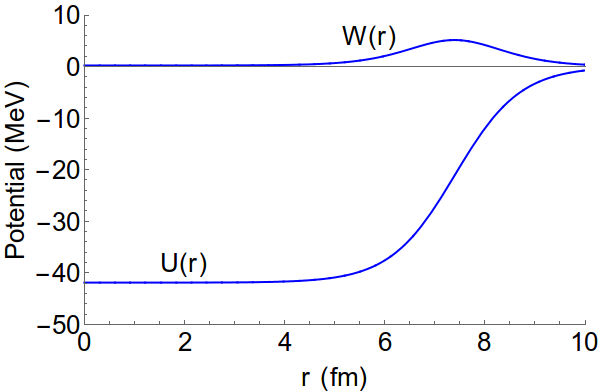
\includegraphics[width=0.35\textwidth]{../fig3_3.png}
      \label{fig:phenpot}
   \end{figure}
\end{itemize}
}

\frame{\frametitle{Optical Model}
\begin{itemize}
   \item Riddle to be solved later. Imagine a 40 MeV neutron begin scattered. By the equations before ($\lambda = 1/2\kappa$) we get $\lambda \approx 5$ fm. However when we use the cross section to calculate it with $\sigma \approx 4\pi d\sigma/d\Omega$ we get
   \begin{equation}
      \lambda = (n\sigma)^{-1} \approx 0.4 \mathrm{fm}.
   \end{equation}
\end{itemize}
}

\end{document}
